% ==============================================================================
% Section 3: The Coordinate Serialization Bottleneck
% ==============================================================================

\section{The Coordinate Serialization Bottleneck}
\label{sec:analysis}

We investigate \emph{where} GUI grounding signals are encoded across transformer layers, progressing from the layerwise spatial profile (Finding~1), through the spatial--serialization dissociation (Finding~2) and its instruction-conditioning (Finding~3), to the resolution-dependent consequence (Finding~4).

\paragraph{Experimental setup.}
We study four GUI agents spanning two backbone families, Qwen2.5-VL~\cite{qwen25vl} and Qwen3-VL~\cite{qwen3vl}, on ScreenSpot-Pro~\citep{screenspotpro} and ScreenSpot-v2~\citep{Os-atlas}.
Spatial grounding quality is measured via a lightweight per-layer grounding head, Stage~1 of \S\ref{sec:method:stage1}, which is under $1\%$ of backbone parameters and is trained with the backbone completely frozen, so it introduces no new spatial knowledge.
Coordinate serialization quality is measured via the backbone's native language model head under teacher forcing, with no additional parameters.

\begin{figure*}[t]
 \centering
 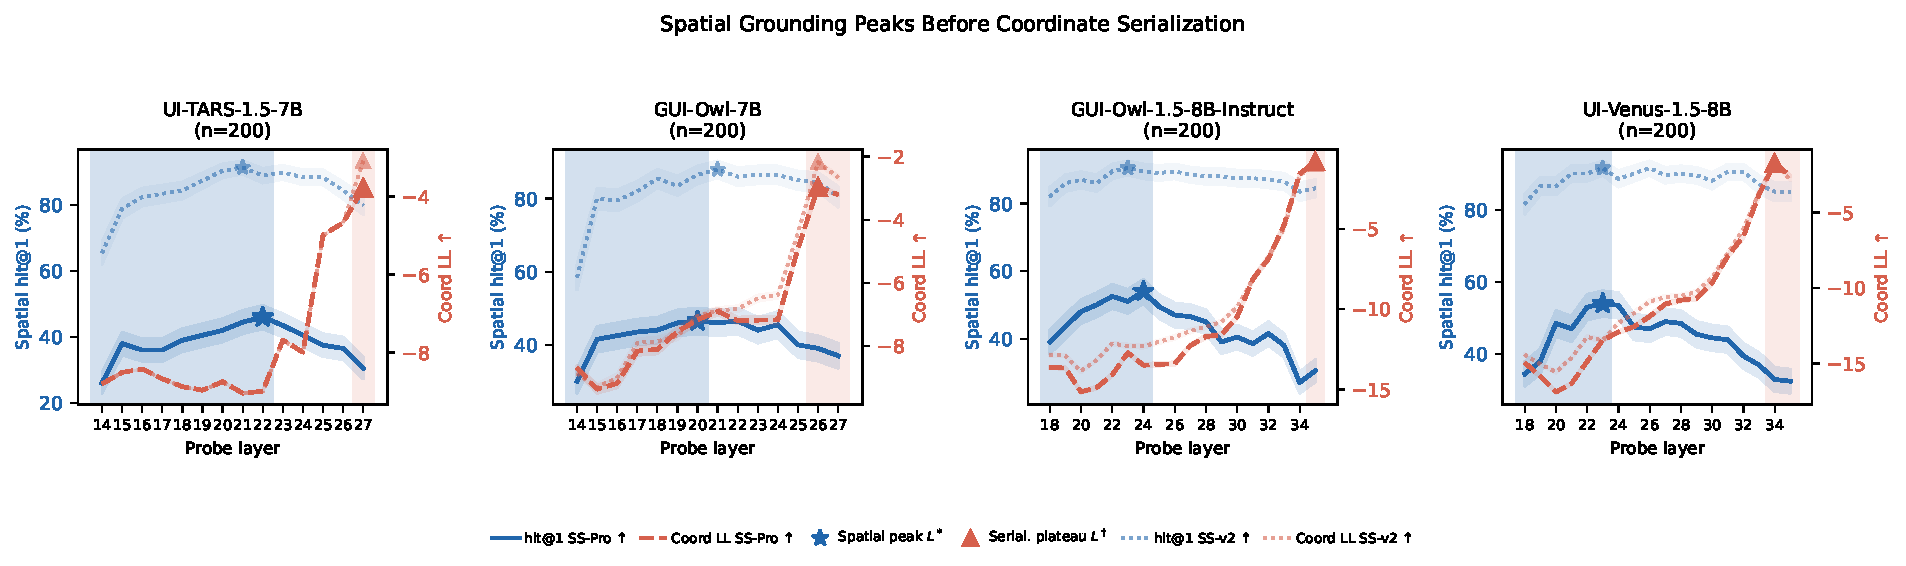
\includegraphics[width=\textwidth]{figs/fig3_serialization_lens.pdf}
 \caption{
 \textbf{Spatial localization and coordinate serialization peak at different depths.}
 Blue curves (left axis): spatial hit@1 $\uparrow$.
 Orange curves (right axis): coordinate token log-likelihood $\uparrow$.
 Both signals rise together, then diverge at the spatial peak $L^*$ (blue star): spatial quality declines while serialization continues rising to $L^\dagger$ (orange triangle).
 The consistent lag $L^\dagger > L^*$ across all models constitutes direct evidence for the coordinate serialization bottleneck.
 }
 \label{fig:serialization_lens}
\end{figure*}

% ------------------------------------------------------------------------------
\subsection{Spatial Grounding Peaks at Intermediate Layers}
\label{sec:analysis:layerwise}
% ------------------------------------------------------------------------------

Autoregressive GUI agents implicitly assume final-layer representations carry the richest spatial information.
The blue curves in Figure~\ref{fig:serialization_lens} challenge this: spatial quality peaks at intermediate depths, then declines toward the output, a non-monotonic trajectory consistent across both backbone families.

\begin{tcolorbox}[colback=gray!8, colframe=gray!40, boxrule=0.4pt, arc=2pt, left=4pt, right=4pt, top=3pt, bottom=3pt]
\textbf{Finding 1.}
\emph{Intermediate transformer layers are consistently better spatial decoders than the final layer.}
\end{tcolorbox}

\paragraph{Robustness.}
The inverted-U is robust to distribution and sample size: across all five benchmarks, $L^*$ varies by $\le 3$ layers per model (std $\le 1.1$), and peak exceeds final in $20/20$ cells.
Bootstrap resampling ($1000$ resamples) places $L^\dagger$ within $\le 1$-layer 95\% CI for every model and $L^*$ within $\le 3$ layers for three of four; $L^* < L^\dagger$ holds in all four.
Full tables are in the supplementary material.

% ------------------------------------------------------------------------------
\subsection{A Dissociation Between Spatial Localization and Coordinate Serialization}
\label{sec:analysis:serialization}
% ------------------------------------------------------------------------------

Finding~1 raises the question: if late layers are not spatial refiners, what do they do?
We hypothesize they specialize in \emph{coordinate serialization}---translating a latent spatial intent into the vocabulary-level token sequence.
We test this with a \emph{serialization lens}: coordinate-token log-likelihood measured via teacher forcing at each layer.

The orange curves in Figure~\ref{fig:serialization_lens} reveal a dissociation: both signals rise together through early layers, then diverge---spatial quality peaks and falls while coordinate log-likelihood continues climbing to a later plateau.
The lag $L^\dagger > L^*$ is consistent across all four models and both backbone families, constituting direct evidence for a \textbf{coordinate serialization bottleneck}.


\begin{tcolorbox}[colback=gray!8, colframe=gray!40, boxrule=0.4pt, arc=2pt, left=4pt, right=4pt, top=3pt, bottom=3pt]
\textbf{Finding 2.}
\emph{The layer that best decodes the target region consistently precedes the layer that best predicts the coordinate token sequence. Late layers are coordinate serializers, not spatial refiners.}
\end{tcolorbox}

\paragraph{Logit-lens controls.}
Applying the native LM head to intermediate states is a logit-lens-style probe~\citep{nostalgebraist2020logitlens}; late layers could align better with the output space for reasons unrelated to coordinates~\citep{geva2021transformer,meng2022locating}. Two controls address this; full tables are in the supplementary material.

\emph{Non-coordinate control.}
We repeat the teacher-forced measurement on \emph{non-coordinate} protocol tokens (parentheses, JSON keys) from the same generations. These reach near-zero NLL at late layers for three of four models, confirming generic alignment. Crucially, coordinate \emph{value} tokens retain a substantial residual NLL at the plateau ($2.2$--$3.1$\,nats for Qwen2.5-VL; $1.0$--$1.7$\,nats for Qwen3-VL), even where format tokens are fully serialized. This residual is the coordinate-specific bottleneck component. The plateau $L^\dagger$ coincides for coordinate and protocol tokens in 3/4 models, so $L^\dagger$'s \emph{location} is a general late-layer phenomenon while the coordinate-specific signal is the residual gap.

\emph{Tuned-lens control.}
Following~\citep{belrose2023tunedlens}, we fit a per-layer affine map to the final-layer representation and apply the \emph{frozen} output head. Calibration flattens the raw trend (early-layer NLL: $8.6\to 3.8$ nats), showing part of the raw improvement is an alignment artifact. The plateau layer, however, is unchanged (L26 both before and after), so the \emph{locus} is robust. Together, the residual NLL gap and the calibration-invariant plateau indicate genuine coordinate serialization.

% ------------------------------------------------------------------------------
\subsection{The Mid-Layer Posterior Is Instruction-Conditioned, Not Visual Saliency}
\label{sec:analysis:counterfactual}
% ------------------------------------------------------------------------------

An alternative is that mid-layer spatial signals merely reflect \emph{visual saliency}. To test this, we design a counterfactual: for pairs sharing the same screen but targeting disjoint elements, we swap the instruction while keeping the image fixed.

Figure~\ref{fig:counterfactual} shows the posterior shifts dramatically: switching the instruction collapses the spatial mass on the original target, concentrated at exactly the intermediate layers where grounding peaks. This rules out the saliency account.

\begin{figure*}[t]
 \centering
 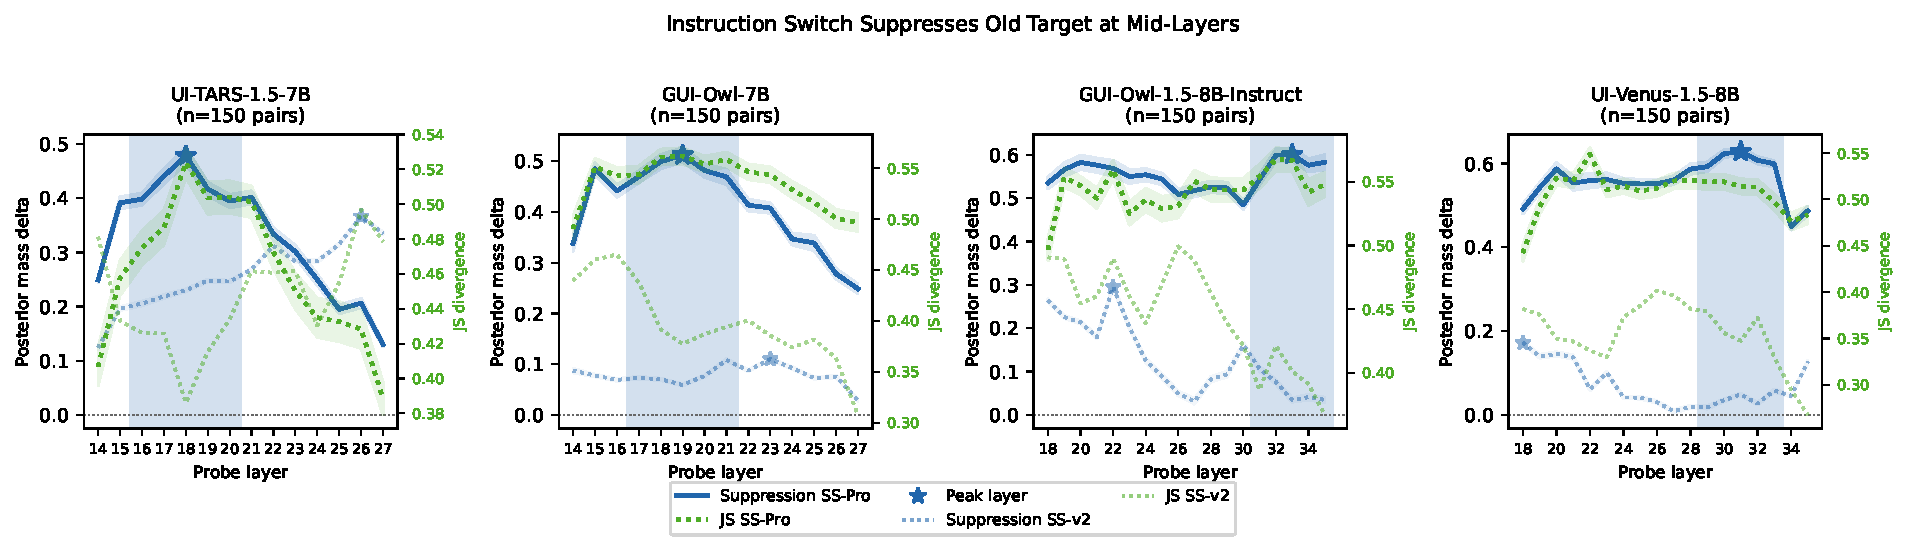
\includegraphics[width=\textwidth]{figs/fig4_instruction_suppression.pdf}
 \caption{
 \textbf{Instruction-switch counterfactual: the mid-layer posterior is instruction-conditioned.}
 Blue curves: old-target suppression $\uparrow$.
 Orange curves: posterior JS divergence $\uparrow$.
 Both effects peak at the same intermediate layers as spatial grounding quality (cf.\ Fig.~\ref{fig:serialization_lens}) and are substantially nonzero, ruling out visual saliency.
 }
 \label{fig:counterfactual}
\end{figure*}

\begin{tcolorbox}[colback=gray!8, colframe=gray!40, boxrule=0.4pt, arc=2pt, left=4pt, right=4pt, top=3pt, bottom=3pt]
\textbf{Finding 3.}
\emph{Swapping the instruction while keeping the image fixed causes a large shift in the mid-layer spatial posterior. The spatial signal is instruction-conditioned grounding, not visual saliency.}
\end{tcolorbox}

% ------------------------------------------------------------------------------
\subsection{The Bottleneck Is More Consequential on High-Resolution, Fine-Grained Layouts}
\label{sec:analysis:resolution}
% ------------------------------------------------------------------------------

Finally, we ask whether the bottleneck is more consequential where GUI grounding is hardest---high-resolution screenshots with small, densely packed targets.

We quantify severity via the \emph{collapse gap}: peak-layer hit@1 minus final-layer hit@1.
Table~\ref{tab:resolution_comparison} shows the gap is consistently larger on ScreenSpot-Pro than on ScreenSpot-v2 across every model.

\begin{table}[t]
\centering
\small
\setlength{\tabcolsep}{4pt}
\begin{tabular}{lrrr@{\hspace{0.8em}}rrr}
\toprule
& \multicolumn{3}{c}{SS-Pro} & \multicolumn{3}{c}{SS-v2} \\
\cmidrule(lr){2-4} \cmidrule(lr){5-7}
Model & Pk$_{\text{probe}}$ & Fin$_{\text{probe}}$ & Gap$\downarrow$ & Pk$_{\text{probe}}$ & Fin$_{\text{probe}}$ & Gap$\downarrow$ \\
\midrule
UI-TARS-1.5-7B & 46.0 & 30.5 & 15.5 & 91.5 & 80.0 & 11.5 \\
GUI-Owl-7B & 46.5 & 37.0 & 9.5 & 88.0 & 80.5 & 7.5 \\
GUI-Owl-1.5-8B & 54.0 & 30.5 & 23.5 & 90.5 & 84.5 & 6.0 \\
UI-Venus-1.5-8B & 54.0 & 32.5 & 21.5 & 91.5 & 85.0 & 6.5 \\
\bottomrule
\end{tabular}
\caption{
 \textbf{Collapse gap is larger on high-resolution layouts.}
 Pk$_{\text{probe}}$ and Fin$_{\text{probe}}$ are the peak-layer and final-layer \emph{spatial-probe} hit@1 (pp) from \S\ref{sec:analysis:layerwise}, not the backbone's native autoregressive accuracy reported as ``Native'' in Table~\ref{tab:main_ensemble}; the two tables use different metrics (hit@1 here vs.\ overlap@1 there) and different readouts (probe vs.\ native decoder).
 SS-Pro gaps consistently exceed SS-v2 gaps.
}
\label{tab:resolution_comparison}
\end{table}

\paragraph{Controlled within-benchmark target-size regression.}
SS-Pro vs SS-v2 conflates target size with resolution. To isolate size, we hold the benchmark fixed at ScreenSpot-Pro ($n{=}1581$) and bin by target bbox area (supplementary material). The peak--final \emph{gap} does \emph{not} increase monotonically as targets shrink: it rises for the two Qwen2.5-7B models but peaks at intermediate sizes for the Qwen3-8B models, floored by peak accuracy on sub-patch targets. Absolute final-layer hit@1, however, is $\sim$1.7$\times$ worse on the smallest quintile ($\sim$34\% vs $\sim$58\%), so the bottleneck is most damaging in absolute terms on small targets even though the gap is not monotone in size.

\begin{tcolorbox}[colback=gray!8, colframe=gray!40, boxrule=0.4pt, arc=2pt, left=4pt, right=4pt, top=3pt, bottom=3pt]
\textbf{Finding 4.}
\emph{The collapse gap is larger on high-resolution ScreenSpot-Pro than on mid-resolution ScreenSpot-v2. Within ScreenSpot-Pro, final-layer accuracy is lowest on the smallest targets even though the collapse gap is not monotone in target size; the bottleneck is most consequential, though not largest in gap, for fine-grained layouts.}
\end{tcolorbox}

Taken together, the four findings motivate reading the spatial posterior from intermediate layers and using cross-layer fusion to select the optimal depth per sample, as described below.
